
%-------------------------------------------------------
%--------------------- Assignment 1 Appendix -----------
%-------------------------------------------------------
\section{Assignment 1 images}
\subsection{Boston Housing}
\label{app:boston_housing}

\begin{figure}[H]
\centering
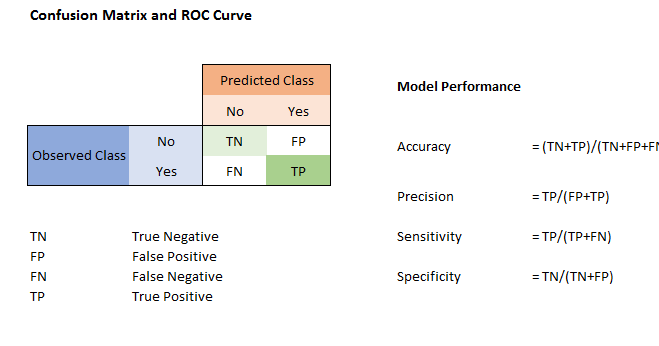
\includegraphics[scale=0.55]{Graphics/Assignment1/ConfusionMatrix.png}
\caption{Confusion Matrix}
\label{fig:confusion_Matrix}
\end{figure}

\subsection{LDA coefficients results}
\begin{figure}[H]
\centering
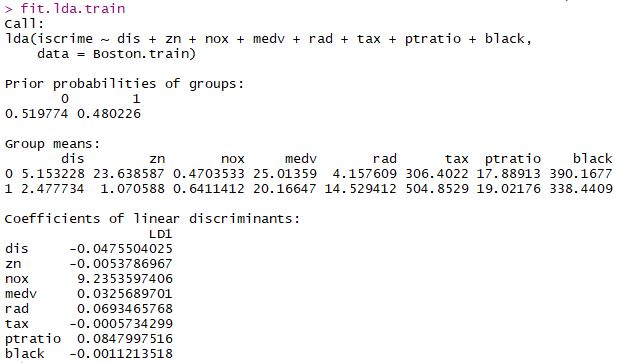
\includegraphics[scale=0.55]{Graphics/Assignment1/LDACoefficients_005.JPG}
\caption{Coefficients for significance level 5\%}
\label{fig:coefficients_method_005}
\end{figure}

\begin{figure}[H]
\centering
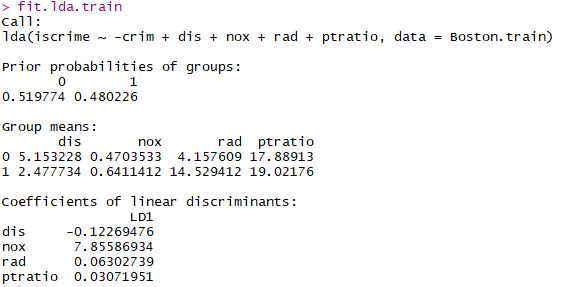
\includegraphics[scale=0.55]{Graphics/Assignment1/LDACoefficients_001.JPG}
\caption{Coefficients for significance level 1\%}
\label{fig:coefficients_method_001}
\end{figure}

\begin{figure}[H]
\centering
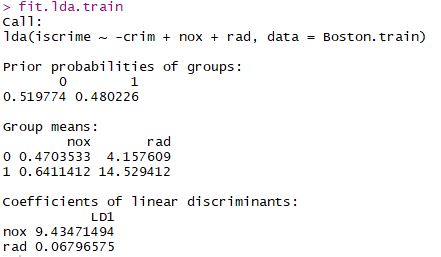
\includegraphics[scale=0.55]{Graphics/Assignment1/LDACoefficients_0001.JPG}
\caption{Coefficients for significance level 0.1\%}
\label{fig:coefficients_method_0001}
\end{figure}

\begin{figure}[H]
\centering
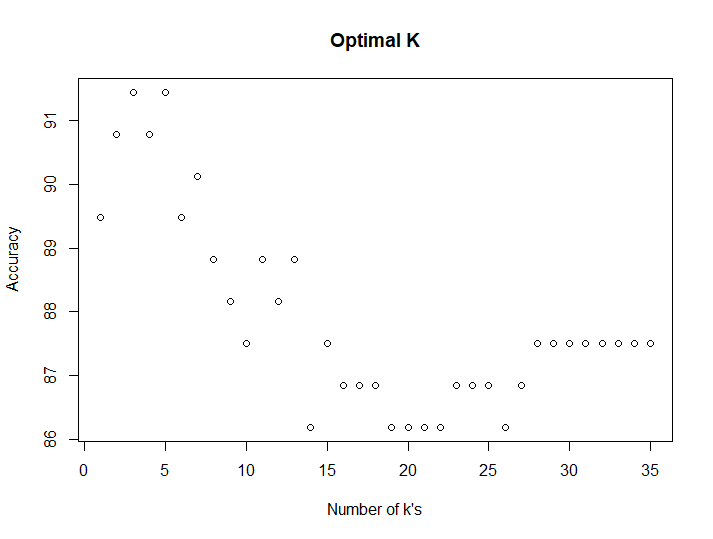
\includegraphics[scale=0.5]{Graphics/Assignment1/Rplot.png}
\caption{Plot of all k's}
\label{app:optimal_ks}
\end{figure}

\lstinputlisting[label={lst:Q1_Boston_Housing}, caption={R script for Q1 Boston Housing}, language={R}]{Graphics/Assignment1/Q1_Boston_Housing2.R}

\subsection{Students Performance}
\label{app:students_performance}

\begin{align*}
    \mathbb{P}(\Pi_1 | \textbf{x}) = \frac{e^{L(\textbf{x})}}{1+e^{L(\textbf{x})}} &= 0.8 \\
    e^{L(\textbf{x})} &= 0.8 \cdot (1+e^{L(\textbf{x})}) \\
    e^{L(\textbf{x})} &= 0.8 + 0.8 \cdot e^{L(\textbf{x})} \\
    -0.8 &= 0.8 \cdot e^{L(\textbf{x})} - e^{L(\textbf{x})} \\ 
    -0.8 &= -0.2 \cdot e^{L(\textbf{x})} \\
    \frac{-0.8}{-0.2} &= e^{L(\textbf{x})} \\
    ln(\frac{-0.8}{-0.2}) &= L(\textbf{x}) = 1.386 \\
    & \\
    L(\textbf{x}) = -6+[0.05,1]\begin{bmatrix}x_1 \\ 3.5\end{bmatrix}&=1.386 \\
    -6+0.05 \cdot x_1+1 \cdot 3.5&=1.386\\
    0.05 \cdot x_1&=1.386+6-3.5\\
    x_1=\frac{3.886}{0.05}&=77.72 hours \\
\end{align*}

%-------------------------------------------------------
%--------------------- Assignment 2 Appendix -----------
%-------------------------------------------------------
\section{Assignment 2 images}
\label{app:alcohol_related_car_crashes}

\begin{figure}[H]
    \centering
    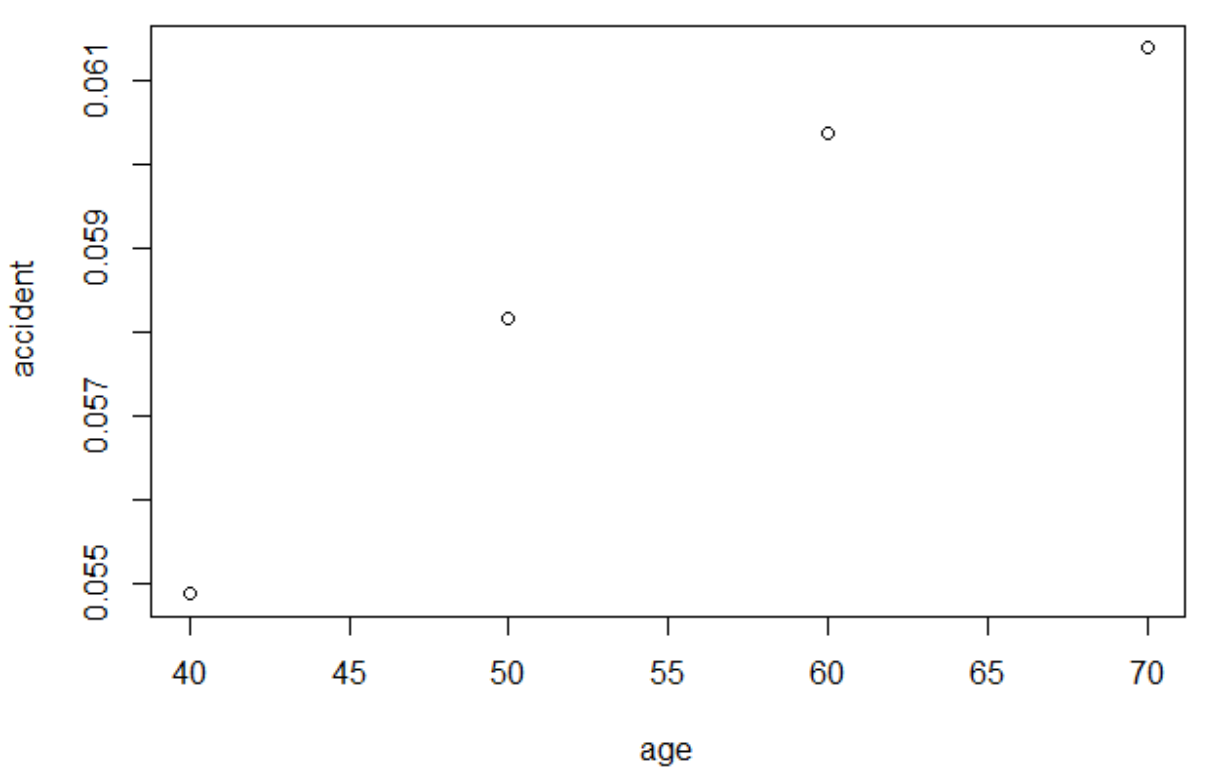
\includegraphics[scale=0.5]{difference_of_ages.PNG}
    \caption{Differences in accidents by ages}
    \label{fig:differences_in_ages}
\end{figure}

\lstinputlisting[label={lst:alcohol_related}, caption={R script for alcohol related car crashes}, language={R}]{Graphics/Assignment2/alcoholRelatedCarCrashes.R}


%-------------------------------------------------------
%--------------------- Assignment 3 Appendix -----------
%-------------------------------------------------------
\section{Assignment 3 images}
\label{app:artist_identification}
%--------------- Renoir Image -------------------------
\begin{figure}[H]
    \centering
    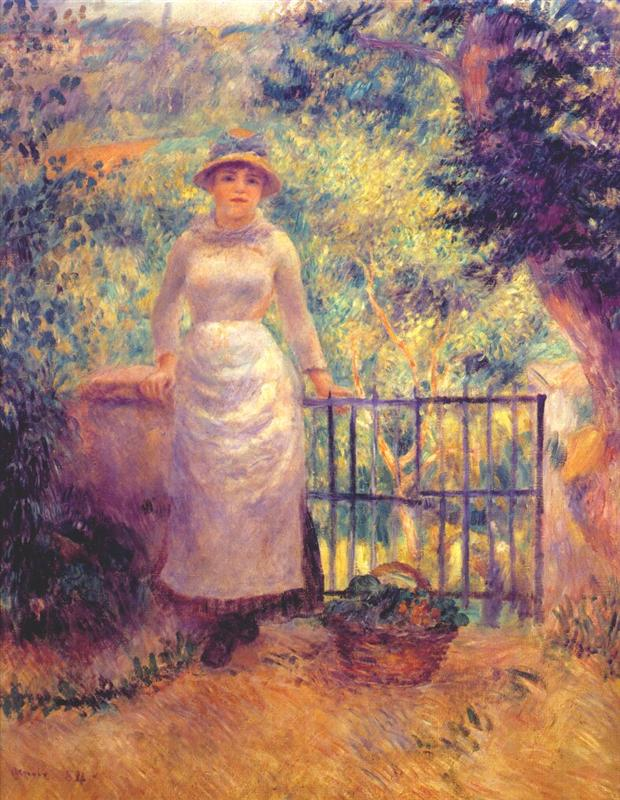
\includegraphics[scale=0.3]{Graphics/Assignment3/renoir.png}
    \caption{Pierre-Auguste Renoir: Aline at the gate.}
    \label{fig:renoir}
\end{figure}
%--------------- Outlier Image -------------------------

\begin{figure}[H]
    \centering
    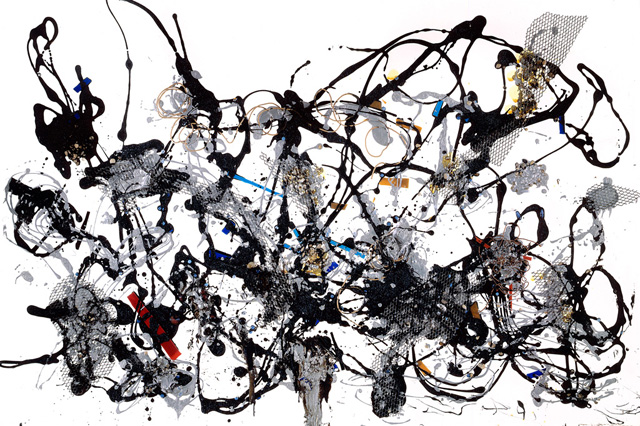
\includegraphics[scale=0.5]{Graphics/Assignment3/outlier.png}
    \caption{Jackson Pollock: Number 29.}
    \label{fig:outlier}
\end{figure}

%--------------- Manet Image -------------------------
\begin{figure}[H]
    \centering
    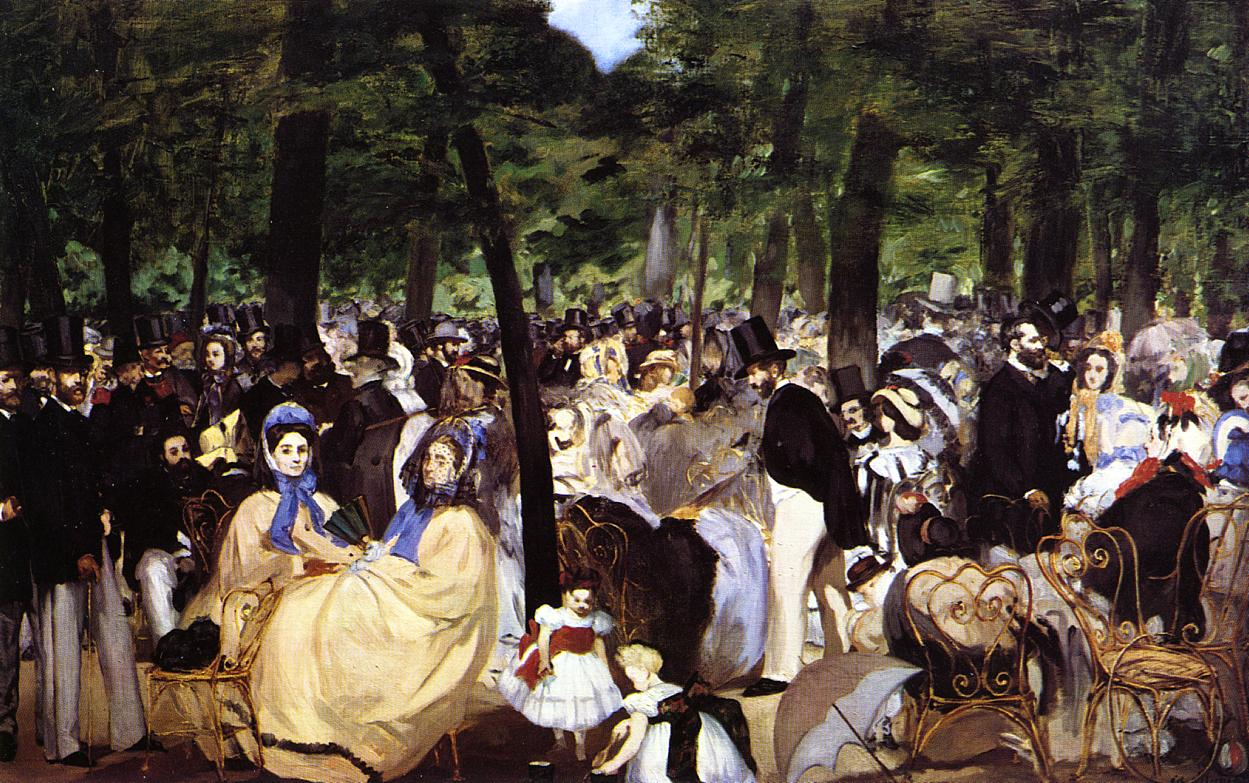
\includegraphics[scale=0.3]{Graphics/Assignment3/manet.png}
    \caption{Édouard Manet: Music in the Tuileries.}
    \label{fig:manet}
\end{figure}


%--------------- Degas Image -------------------------

\begin{figure}[H]
    \centering
    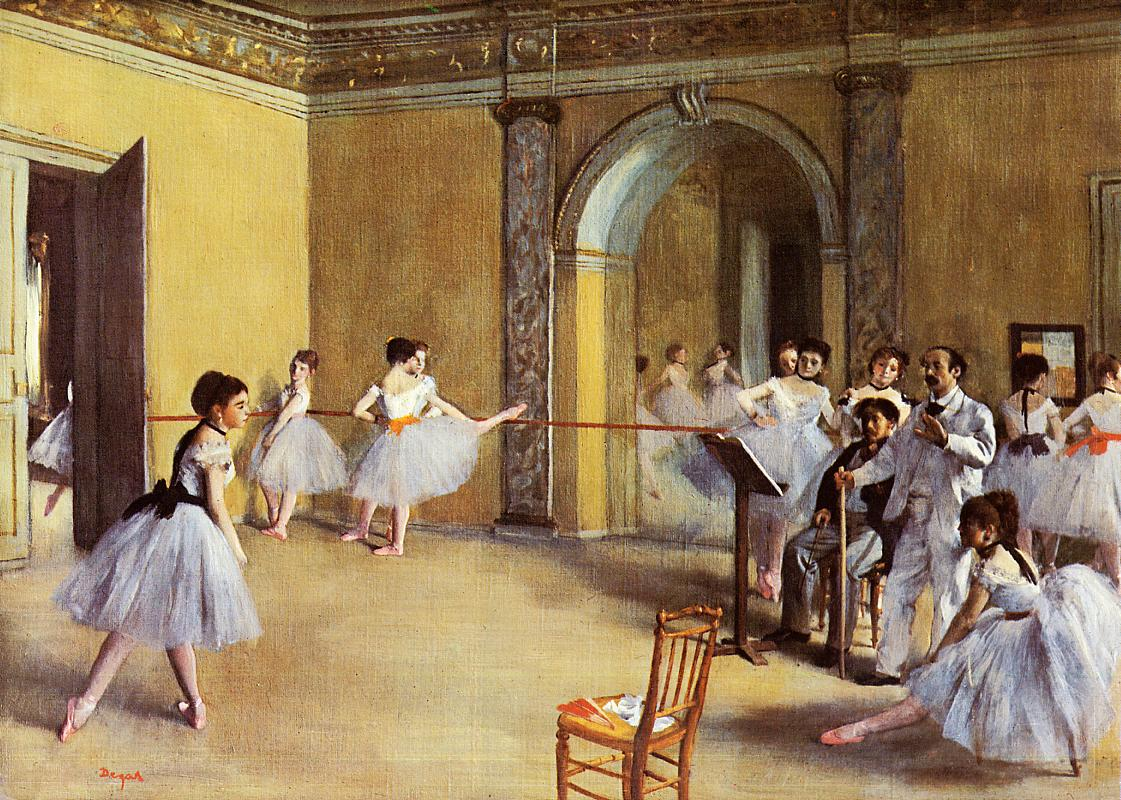
\includegraphics[scale=0.3]{Graphics/Assignment3/degas.png}
    \caption{Edgar Degas: Dance Class at the Opera.}
    \label{fig:degas}
\end{figure}

%--------------- VGG16 model Image -------------------------

\begin{figure}[H]
    \centering
    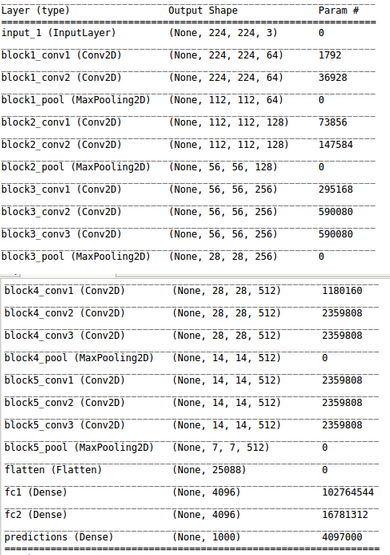
\includegraphics[scale=0.7]{Graphics/Assignment3/VGG16_model_image.png}
    \caption{VGG16 model with 1000 classes as output.}
    \label{fig:imagenet_vgg16}
\end{figure}

%--------------- Custom VGG16 model Image -------------------------

\begin{figure}[H]
    \centering
    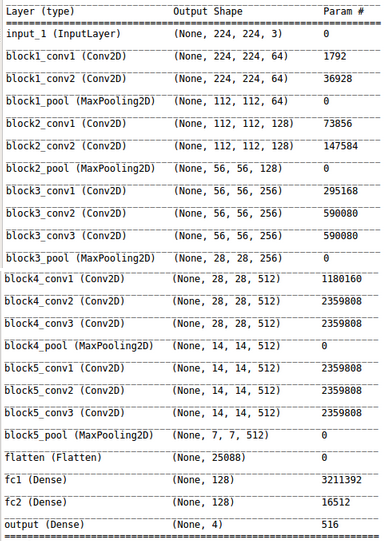
\includegraphics[scale=0.7]{Graphics/Assignment3/custom_model_image.png}
    \caption{Custom VGG16 model with 4 classes as output.}
    \label{fig:custom_vgg16}
\end{figure}

\section{Assignment 3 code}

%------------------ Fetch image code ----------------------
\begin{lstlisting}[frame=single, language=Bash, label={code:fetch_images}, caption={Code to fetch images from Wikiart for specific artists, in this case Manet.}]
    curl -s "https://www.wikiart.org/en/App/Painting/PaintingsByArtist?artistUrl=edouard-manet&json=2" | jq -r 'map(.image) | join("\n")' | sed '' | xargs -P 10 -n 1 curl -s -O
\end{lstlisting}

%------------------ Load data for preprocessing ---------------
\begin{lstlisting}[frame=single, language=Python, label={code:load_data}, caption={Code to load data for preprocessing.}]
    for dataset in data_dir_list:
	    image_list=os.listdir(data_path+'/'+ dataset)
    	for image in image_list:
    		image_path = data_path + '/'+ dataset + '/'+ image 
    		image = image.load_image(image_path, target_size=(224, 224))
    		img = image.image_to_array(image)
    		img = np.expand_dimensions(img, axis=0)
    		img = preprocess_input(img)
    		image_data_list.append(img)
\end{lstlisting}


%------------------- Shuffle and split into training and test --------------------
\begin{lstlisting}[frame=single, language=Python, label={code:shuffle_and_split_data}, caption={Code to shuffle and split the data to 80\% training and 20\% test.}]
# Split the dataset
X_train, X_test, y_train, y_test = train_test_split(image_data, Y, test_size=0.2, random_state=2)
\end{lstlisting} 

\begin{lstlisting}[frame=single, language=Python, label={code:model_creation_and_training}, caption={Code to load VGG16 pre-trained on ImageNet and doing transfer learning.}]
# Adjust the image input to 224, 224 and 3 channels
image_input = Input(shape=(224, 224, 3))

# VGG16 model
imagenet_model = VGG16(input_tensor=image_input, include_top=True,weights='imagenet')

# Get VGG16's block5_pool layer and take its output
last_layer = imagenet_model.get_layer('block5_pool').output
# Feed the output of block5_pool to the Flatten layer
x= Flatten(name='flatten')(last_layer)
# Create two fully connected layers with 128 neurons each, using RELU activation
x = Dense(128, activation='relu', name='fc1')(x)
x = Dense(128, activation='relu', name='fc2')(x)
# Create a output layer, using softmax classification
output_layer = Dense(num_classes, activation='softmax', name='output')(x)
# Assign the new model to a variable
custom_model = Model(image_input, output_layer)

# Freeze all the layers except the dense layers that was created above
for layer in custom_model.layers[:-3]:
	layer.trainable = False

# Compile the new model architecture
custom_model.compile(loss='categorical_crossentropy',optimizer='adadelta',metrics=['accuracy'])

# Train the model for 20 epochs using a batch size of 4
custom_model.fit(X_train, y_train, batch_size=4, epochs=20, verbose=1, validation_data=(X_test, y_test))

# Test the model using accuracy as a metric
(loss, accuracy) = custom_model.evaluate(X_test, y_test, batch_size=10, verbose=1)
print('loss={:.4f}, accuracy: {:.4f}%'.format(loss,accuracy * 100))
\end{lstlisting}



